\documentclass[a4paper]{article}

\usepackage{amsmath}
\usepackage{amssymb}
\usepackage{stellar}
\usepackage{parskip}
\usepackage{fullpage}
\usepackage{wrapfig}
\usepackage{tikz}

\usetikzlibrary{cd}

\title{Probability}
\author{Paolo Bettelini}
\date{}

\begin{document}

\maketitle
\tableofcontents

\pagebreak

\section{Probabilità}

\subsection{Costruzione intuitiva}

\begin{radioactive}
\sexample{Approccio classico alla probabilità}{
    Consideriamo un'urna contenente 6 palline numerate da \(1\) a \(6\) e per il resto indistinguibili.
    Vogliamo studiare l'esperimento estrazione di una pallina dall'urna.
    Voglio studiare quale pallina sia più probabile che venga estratta.
    Vogliamo quindi mettere un ordinamento sull'insieme degli eventi di questo esperimento.
    Sia \(\Omega\) l'insieme di tutti i possibili risultati dell'esperimento.
    Sia \(P_i\) la probabilità di estrarre il numero \(i \in \{1,2,3,5,6\}\).
    In questo caso la scelta naturale è \(P_i = \frac16\) per tutte le \(i \in \{1,2,3,4,5,6\}\).
    Notiamo che \(\sum P_i = 1\), cioè la probabilità di estrarre un numero da \(1\) a \(6\), cioè in questo
    caso l'evento certo. Questa viene detta additività della probabilità di eventi disgiunti.
    Inoltre, la probabilità \(P_j = 0\) con \(j \notin \{1,2,3,4,5,6\}\).
    Possiamo anche notare che
    \[
        P_i = \frac{\text{Casi favorevoli}}{\text{Casi possibili}}
        = \frac{
            |\{i\}|
        }{|N|}
    \]
    In questo caso i casi elementari \(\{i\}\) sono equiprobabili.
}
\end{radioactive}

\begin{radioactive}
\sexample{Approccio frequentista alla probabilità}{
    Consideriamo l'esperimento lancio di un dado
    a 6 facce numerate da \(1\) a \(6\).
    Abbiamo \(\Omega = \{1,2,3,4,5,6\}\).
    In questo caso non è detto che gli eventi o i casi elementari
    siano equiprobabili. Quindi,
    per assegnare i \(P_i\) potremmo lanciare il dado sperimentalmente.
    \[
        P_i^{(k)} = \frac{N_i^{(k)}}{k}
    \]
    con \(N_i^k\) è il numero di volte che esce l'evento \(i\) su \(k\) lanci.
    Chiaramente questi valori sono variabili, quindi prendiamo
    \[
        P_i = \lim_{k \to +\infty} P^{(k)}_i
    \]
    per  \(i \in \{1,2,3,4,5,6\}\) se il limite esiste.
    Notiamo che \(P_i^{(k)} \in [0,1]\) e
    \[
        \sum_{i=1}^6 P_i^{(k)} = 1, \quad k \in \naturalnumbers
    \]
    e prendendo il limite \(k \to +\infty\)
    \[
        \sum_{i=1}^6 P_i = 1
    \]
}
\end{radioactive}

\begin{radioactive}
In entrambi i casi abbiamo quindi le medesime proprietà
ma nella seconda le probabilità non coincidono necessariamente.
\end{radioactive}

\begin{radioactive}
\sexample{Probabilità soggettiva}{
    Consideriamo un torneo di calcio dove tutti giocano contro tutti, in cui partecipano 6 squadre:
    (1) R. Madrid, (2) M. City, (3) Bayer Monaco, (4) Atalanta, (5) Porto, (6) Nantes.
    L'esperimento che consideriamo è quello che studia il vincitore del torneo.
    Abbiamo \(\Omega = \{1,2,3,4,5,6\}\).
    L'approccio classico richiede casi elementari equiprobabili, e in questo caso non lo sono.
    L'approccio frequentista richiede di richiedere un torneo molte volte sotto le stesse condizioni,
    il che è praticamente impossibile.
    L'idea alternativa è quindi quella di chiedere a due esperti del settore
    di assegnare le probabilità in maniera coerente alle osservazioni che abbiamo
    fatto negli altri due approcci.
    Il primo esperto scegli per esempio \[
        P_1 = \frac14,
        P_2 = \frac14,
        P_3 = \frac15,
        P_4 = \frac15,
        P_5 = \frac{1}{10},
        P_6 = 0
    \]
    mentre il secondo \[
        P_1 = \frac{11}{27},
        P_2 = \frac13,
        P_3 = \frac19,
        P_4 = \frac{2}{27},
        P_5 = \frac{1}{27},
        P_6 = \frac{1}{27}
    \]
    Chiaramente c'è natura soggettiva.
}
\end{radioactive}

\begin{radioactive}
\sdefinition{Probabilità soggettiva}{
    Si definisce probabilità di un evento
    la misura del grado di fiducia, cioè un numero reale in \([0,1]\),
    che in individuo coerente
    assegna al verificarsi dell'evento considerato, in base alle sue conoscenze. \\
    In altro modo, la probabilità di un evento è quanto un individuo coerente ritiene equo pagare
    per ricevere \(1\) se l'evento si verifica e \(0\) se non si verifica.
}
\end{radioactive}

\begin{radioactive}
Ognuno degli approcci ricopre l'approccio precedente.
Quello soggettivo è quello più generale.
\end{radioactive}

\subsection{Formalizzazione}

\begin{radioactive}
\sdefinition{Esito}{
    Un \emph{esito} è una qualsiasi asserzione
    della quale ne si può stabilire la veridicità
    osservando il risultato dell'esperimento. 
}
\end{radioactive}

\begin{radioactive}
Se abbiamo un urna possiamo rappresentare
gli eventi come punti su un segmento di punti, cioè tutte le possibili estrazioni.
Con due urne posso fare lo stesso con una griglia discreta, e così via.
\end{radioactive}

\begin{radioactive}
\sdefinition{Evento}{
    Un \emph{evento} è un insieme di esiti.
}
\end{radioactive}

Possiamo fare un ponte fra gli operatori della teoria degli insiemi e
la logica degli eventi.

% logic-of-probability-events-definition
Siano \(A, B\) due eventi, indicati con i rispettivi insiemi di esiti \(A\) e \(B\).
\begin{enumerate}
    \item La \emph{negazione} di un evento \(-A\) corrisponde all'evento associato all'insieme complementare \(\Omega \difference A\).
    \item La \emph{somma} logica di due eventi \(A+B\), cioè se almeno uno dei due eventi si verificano, corrisponde all'evento associato all'unione insiemistica \(A \union B\).
    \item Il \emph{prodotto} logico di due eventi \(A\cdot B\), cioè se ambo gli avventi si verificano, corrisponde all'evento associato all'intersezione insiemistica \(A \intersection B\).
    \item La \emph{differenza} logica di due eventi \(A - B\) corrisponde all'evento associato alla differenza insiemistica \(A \difference B\). 
    \item La \emph{differenza simmetrica} di due eventi \(A\Delta B\) corrisponde all'evento associato alla differenza simmetrica insiemistica \((A \intersection B^c) \union (A^c \intersection B)\).
    \item L'\emph{implicazione} logica di due eventi \(A\implies B\) corrisponde all'evento associato alla relazione di sottoinsieme \(A \subseteq B\).
    \item L'\emph{equivalenza} fra due eventi \(A = B\), cioè \(A \implies B\) e \(B \implies A\), corrisponde all'uguaglianza insiemistica \(A = B\).
    \item Due eventi si dicono \emph{incompatibili}, cioè se non possono verificarsi in contemporanea, corrisponde alla condizione che l'intersezione insiemistica sia vuota \(A \intersection B = \emptyset\).
\end{enumerate}

La teoria degli insiemi non è esattamente la stessa cosa della teoria degli eventi.
Per esempio la probabilità condizionata non corrisponde a nessun insieme.


\sdefinition{}{
    Nel caso della probabilità classica con \(\Omega\) finito, possiamo scegliere l'insieme
    degli eventi come \(\powerset(\Omega)\)
    e definire la misura come \(\mathbb P \colon \powerset(\Omega) \fromto [0,1]\) dato da
    \[
        \mathbb P (A) = \frac{|A|}{|\Omega|}
    \]
    per uno spazio equiprobabile.
}

Vogliamo espandersi al caso della probabilità soggettiva
\sdefinition{}{
    Sia \(\Omega \neq \emptyset\) di cardinalità finita.
    Chiamiamo \emph{misura di probabilità} su \(\powerset(\Omega)\)
    una funzione \(\mathbb P \colon \powerset(\Omega) \fromto [0,1]\)
    tale che
    \begin{enumerate}
        \item \(\mathbb P(\Omega) = 1\)
        \item \(\forall A, B \in \powerset(\Omega)\) disgiunti,
        \[  \mathbb P (A \union B) = \mathbb P (A) + \mathbb P (B) \]
    \end{enumerate}
    Chiamiamo \emph{spazio di probabilità con spazio campionato \(\Omega\)
    di cardinalità finita} la terna \((\Omega, \powerset(\Omega), \mathbb P)\).
}

\sproposition{}{
    Sia \((\Omega, \powerset(\Omega), \mathbb P)\)
    uno spazio di probabilità con spazio campionato \(\Omega\)
    di cardinalità finita. Allora,
    \begin{enumerate}
        \item per ogni \(A \in \powerset(\Omega)\), \(\mathbb P(\Omega \difference A) = 1 - \mathbb P (A)\);
        \item per ogni \(A,B \in \powerset(\Omega)\) tale che \(B \subseteq A\),
            \(\mathbb P(A \difference B) = \mathbb P (A) - \mathbb P (B)\)
        \item per ogni \(A,B \in \powerset(\Omega)\), \(\mathbb P (A \union B) = \mathbb P (A) + \mathbb P (B) - \mathbb P (A \intersection B)\)
        \item \emph{Additività:} \(\forall n \in \naturalnumbers\) e \(A_1, \cdots, A_n \in \powerset(\Omega)\) tale che
        \(A_i \intersection A_j = 0\) per tutti gli \(i \neq j\),
        \[
            \mathbb P \left(
                \bigcup_{k=1}^n A_k
            \right) = \sum_{k=1}^n \mathbb P(A_k)
        \]
        \item \emph{Subadditività:} \(\forall n \in \naturalnumbers\) e \(A_1, \cdots, A_n \in \powerset(\Omega)\)
        \[
            \mathbb P \left(\bigcup_{k=1}^n A_k\right) \leq \sum_{k=1}^n \mathbb P(A_k)
        \]
    \end{enumerate}
}

\sproof{}{
    \begin{enumerate}
        \item \begin{align*}
            \mathbb P(\Omega) &= \mathbb P(A \union (\Omega \difference A)) \\
            &= \mathbb P(A) + \mathbb P(\Omega \difference A)
        \end{align*}
        e quindi \(\mathbb P(A) = 1- \mathbb P(\Omega-A)\).
        \item \begin{align*}
            \mathbb P(A \difference B) &= \mathbb P(A \intersection (\Omega \difference B)) = 1- \mathbb P\left(\Omega \difference (A \intersection (\Omega \difference B))\right)
        \end{align*}
        dal disegno degli insiemi
        \begin{align*}
            \mathbb P(A \difference B) &= 1-\mathbb P((\Omega \difference A) \union B) \\
            &= 1 - \mathbb P(\Omega \difference A) - \mathbb P(B) \\
            &= \mathbb P(A) - \mathbb P(B)
        \end{align*}
        \item \begin{align*}
            \mathbb P(A \union B) &= \mathbb P((A \difference A \intersection B) \union (B \difference A \intersection B) \union (A \intersection B)) \\
            &= \mathbb P(A \difference A \intersection B) + \mathbb P((B \intersection A \intersection B) \union (A \intersection B)) \\
            &= \mathbb P(A \difference A \intersection B) + \mathbb P(B \intersection A \intersection B) + \mathbb P(A \intersection B) \\
            &= \mathbb P(A) - \mathbb P(A \intersection B) + \mathbb P(B) - \mathbb P(A \intersection B) + \mathbb P(A \intersection B) \\
            &= \mathbb P(A) + \mathbb P(B) - \mathbb P(A \intersection B)
        \end{align*}
        \item Dimostriamo per induzione. Per \(n=2\) vale per la definizione.
        Assumiamo che la proposizione sia vera per \(n\) e mostriamo il passo successivo
        \begin{align*}
            \mathbb P\left(\bigcup_{i=1}^{n+1} A_i\right)
            &= \mathbb P\left(\bigcup_{i=1}^{n+1} A_i\right) \\
            &= \mathbb P\left(\bigcup_{i=1}^{n} A_i\right) + \mathbb P(A_{n+1}) \\
            &= \sum_{i=1}^{n+1} \mathbb P(A_i)
        \end{align*}
        \item Vale lo stesso passo \(n=2\) dello scorso punto
        \begin{align*}
            \mathbb P(A_1 \union A_2) &= \mathbb P(A_1) + \mathbb P(A_2) - \mathbb P(A_1 \intersection A_2) \\
            &\leq \mathbb P(A_1) + \mathbb P(A_2)
        \end{align*}
        poi segue per induzione come il punto scorso.
    \end{enumerate}
}

\pagebreak

\sproposition{Formula di inclusione-esclusione}{
    Sia \((\Omega, \powerset(\Omega), \mathbb P)\)
    uno spazio di probabilità con spazio campionato \(\Omega\)
    di cardinalità finita.
    Prendiamo \(A_1, \cdots, A_n \in \powerset(\Omega)\) con \(n \in \naturalnumbers\).
    Allora,
    \[
        \mathbb P \left(
            \bigcup_{j=1}^n A_j
        \right) = \sum_{k=1}^n \sum_{\substack{i_1, \cdots, i_k \\ \in \{1,\cdots, n\} \\ i_1 \neq i_2 \cdots i_k}}
        (-1)^{k+1} \mathbb P \left(
            \bigcap_{r=1}^k A_{i_r}
        \right)
    \]
    Tutte le possibili intersezione di \(k\) elementi pesati da \(A_1, \cdots, A_n\).
}

\sproof{}{
    Mostriamolo per induzione
    Il caso \(n=2\) segue dal caso banale dimostrato in precedenza, cioè
    \begin{align*}
        \mathbb P(A_1 \union A_2) &=
        \sum_{k=1}^2 \sum_{\substack{i_1, \cdots, i_k \\ \in \{1,2\} \\ i_1 \neq \cdots \neq i_k}} (-1)^{k+1} \mathbb P\left(
            \bigcap_{r=1}^k A_{i_r}
        \right) \\
        &= \sum_{i_1 \in \{1,2\} } \mathbb P(A_{i_1})
        - \sum_{\substack{i_1, i_2 \in \{1,2\} \\ i_1 \neq i_2 }} \mathbb P(A_1 \intersection A_2) \\
        &= \mathbb P(A_1) + \mathbb P(A_2) - \mathbb P(A_1 \intersection A_2)
    \end{align*}
    Supponiamo che la formula funzioni per \(n-1\) e dimosriamolo per \(n\).
    Abbiamo
    \begin{align*}
        \overline A_{n-1} &= \bigcup_{j=1}^{n-1}A_j \\
        \mathbb P\left(
            \bigcup_{j=1}^n A_j
        \right) 
        &= \mathbb P\left(
            \overline A_{n-1} \union A_n
        \right) \\
        &\overset{(n=2)}{=} 
        \mathbb P(\overline A_{n-1}) +\mathbb P(A_n) - \mathbb P \left(\overline A_{n-1} \intersection A_n\right)
    \end{align*}
    Studiamo separamente il primo termine e l'ultimo termine.
    Nel primo abbiamo
    \begin{align*}
        \mathbb P (\overline A_{n-1}) = \mathbb P\left(
            \sum_{k=1}^{n-1} \sum_{\substack{i_1, \cdots, i_k \\ \in \{1,\cdots,n-1\} \\ i_1 \neq \cdots \neq i_k }} (-1)^{k+1} \mathbb P\left(
                \bigcap_{r=1}^k A_{i_r}
            \right)
        \right)
    \end{align*}
    Per l'ultimo termine usiamo il passo \(n-1\)
    \begin{align*}
        \mathbb P\left(
            \overline A_{n-1} \intersection A_n
        \right) &= \mathbb P \left(
            \left[
                \bigcup_{j=1}^{n-1} A_j
            \right] \intersection A_n
        \right) \\
        &= \mathbb P \left(
            \bigcup_{j-1}^{n-1} (A_j \intersection A_n)
        \right) \\
        &= \sum_{k=2}^{n-1}
        \sum_{\substack{ i_1, \cdots, i_k \\ \in \{1,\cdots, n-1\} \\ i_1 \neq \cdots \neq i_k }}
        \mathbb P \left(
            \bigcap_{r=1}^k (A_{i_r} \intersection A_n)
        \right) \\
        &= -\sum_{k=2}^{n} 
        \sum_{\substack{ i_2, \cdots, i_k \\ \in \{1,\cdots, n\} \\ i_1 \neq \cdots \neq i_k \\ \exists j \in \{1, \cdots, k\} \\ \suchthat i_j = n }}
        \mathbb P \left(
            \bigcap_{r=1}^k A_{i_r}
        \right)
    \end{align*}
    Combinando tuto
    \begin{align*}
        \mathbb P \left(
            \bigcup_{j=1}^n A_j
        \right)
        &= \mathbb P (\overline A_{n-1}) + \mathbb P(A_n) - \mathbb P(\overline A_{n-1} \intersection A_n) \\
        &= \mathbb P(A_n) + \sum_{k=2}^{n} 
        \sum_{\substack{ i_2, \cdots, i_k \\ \in \{1,\cdots, n\} \\ i_1 \neq \cdots \neq i_k \\ \exists j \in \{1, \cdots, k\} \\ \suchthat i_j = n }}
        \mathbb P \left(
            \bigcap_{r=1}^k A_{i_r}
        \right) \\
        &+ \sum_{k=1}^{n-1} \sum_{\substack{i_1, \cdots, i_k \\ \in \{1,\cdots, n-1\} \\i_1 \neq \cdots \neq ik }}
        (-1)^{k+1} \mathbb P\left(
            \bigcap_{r=1}^k A_{i_r}
        \right) \\
        &= \sum_{k=1}^n \sum_{\substack{i_1, \cdots, i_k \\ \in \{1, \cdots, n\} \\ i_1 \neq \cdots \neq i_k }}
        (-1)^{k+1} \mathbb P\left(
            \bigcap_{r=1}^k A_{i_r}
        \right)
    \end{align*}
}

Andiamo a rappresentare il nostro spazio M. D. P con un vettore.
Sia \(N \in \naturalnumbers\) e \(\Omega = \{\omega_1, \cdots, \omega_N\}\).
Notiamo che dato \(A \in \powerset (\Omega)\) possiamo sempre rappresentarlo come
\[
    A = \{\omega_{i_1}, \cdots, \omega_{i_k}\}
\]
con \(k \in \{1, \cdots, N\}\) e \(i_1, \cdots, i_k \in \{1, \cdots, N\}\)
con \(i_1 \neq \cdots \neq i_k\).
Da questo segue che
\begin{align*}
    A &= \bigsqcup_{r=1}^k \{\omega_{i_r}\}
\end{align*}
Quindi per l'additività di una generica M.D.P \(\mathbb P \colon \powerset (\Omega) \fromto [0,1]\)
vale
\[
    \mathbb P (A) = \sum_{r=1}^k \mathbb P(\{\omega_{i_r}\})
\]
Abbiamo quindi scritto la misura di un insieme \(A \in \powerset (\Omega)\)
come la somma delle misure dei singoletti che lo compongono.
Ricordiamo che
\[
    \mathbb P (\Omega) = \sum_{i=1}^N \mathbb P(\omega_i) = 1
\]

\sproposition{}{
    Sia \(\Omega \neq \emptyset\) con \(|\Omega| = N\) finito.
    I seguenti 3 insiemi sono in corrispondenza biunivoca
    \begin{enumerate}
        \item \[
            S_N \triangleq \left\{
                (P_1, \cdots, P_N) \in [0,1]^N \suchthat \sum_{i=1}^N P_i = 1
            \right\}
        \]
        \[
            K_{N-1} \triangleq \left\{
                (P_1, \cdots, P_{N_1})
                \in [0,1]^{N-1} \suchthat \sum_{i=1}^{N-1} P_i \leq 1
            \right\}
        \]
        \item \[
            M(\Omega) \triangleq \left\{
                \mathbb P \text{ M. D. P su } (\Omega, \powerset(\Omega))
            \right\}
        \]
    \end{enumerate} 
}

\sproof{}{
    Per la corrispodnenza fra \(S_n\) a \(K_{N-1}\)
    prendo la funzione \(f \colon K_{N-1} \fromto S_N\) data da
    \[
        f(P_1, \cdots, P_{N_1}) \triangleq \left(P_1, \cdots, P_{n-1}, 1- \sum_{i=1}^{N-1} P_i \right)
    \]
    Dimostrazione per esercizio.
    Dimostriamo che \(M(\Omega)\) e \(S_N\) sono in corrispondenza biunivoca.
    Prendiamo \(g \colon M(\Omega) \fromto S_N\) come
    \[
        g(\mathbb P) \triangleq (
            \mathbb P(\{\omega_1\}),
            \cdots,
            \mathbb P(\{\omega_N\})
        )
    \]
    Notiamo che per definizione di misura di probabilità,
    tutti i termini \(\mathbb P(\{\omega_i\}) \in [0,1]\) per tutte le \(i \in \{1, \cdots, N\}\),
    e \[
        \sum_{i=1}^N \mathbb P(\{\omega_i\}) = \mathbb P(\Omega) = 1
    \]
    quindi \(g(\mathbb P) \in S_n\) ed è ben definita.
    La suriettività è data dal fatto che dato \((P_1, \cdots, P_N) \in S_N\)
    basta prendere \(\mathbb P \in M(\Omega)\) tale che
    \(\mathbb P (\{\omega_i\}) \triangleq P_i\).
    Per l'iniettività prendiamo \(\mathbb P_1, \mathbb P_2 \in M(\Omega)\)
    tali che \(g(\mathbb P_1) = g(\mathbb P_2)\), cioè \(\mathbb P_1(\{\omega_i\}) = \mathbb P_2(\{\omega_i\})\).
    Ma sono uguali in quanto dato \(A = \{\omega_{i_1}, \cdots, \omega_{i_k}\} \in \powerset(\Omega)\)
    \[
        \mathbb P_1(A)
        = \sum_{r=1}^k \mathbb P_1(\{\omega_{i_r}\})=
        \sum_{r=1}^k \mathbb P_2(\{\omega_{i_r}\})
        = \mathbb P_2(A)
    \]
}

Per questa corrispodnenza biunivoca
sono essenziali il possesso di un sottoinsieme di elementi di \(\powerset(\Omega)\)
che genera (tramite unioni ed intersezioni) tutto \(\powerset(\Omega)\),
e pure l'additività (o caso generale sigma additività per il caso infinito).
È importante notare che una funzione generica \(\powerset(\Omega) \fromto [0,1]\)
non è univocamente determinata dal valore che assume sui singoletti.

\section{Indipendenza e condizionamento}











\pagebreak

\section{Temp analisi III}

\stheorem{Criterio di Cauchy}{
    Una successione di funzioni \(\{f_n\}\) converge uniformemente a \(f \colon S \fromto \realnumbers\)
    in \(S\) se e solo se per ogni \(\varepsilon > 0\) esiste \(N(\varepsilon)\) naturale tale che
    \[
        \forall m,n > N,
        |f_n(x) - f_m(x)| < \varepsilon, \forall x \in S
    \]
}

\sproof{}{
    \iffproof{
        Fissiamo \(\varepsilon > 0\).
        Dalla definizione di convergenza uniforme,
        esiste \(N\left(\frac{\varepsilon }{2}\right)\) tale che
        \[
            \left|f_n(x) - f(x)\right| < \frac{\varepsilon}{2}
        \]
        per ogni \(n > N\) e \(x \in S\).
        Quindi, \begin{align*}
            \left|f_n(x) - f(x)\right| &\leq \left|f_n(x) - f(x)\right| + \left|f_n(x) - f(x)\right| \\
            &\leq \frac{\varepsilon}{2} + \frac{\varepsilon}{2} = \varepsilon
        \end{align*}
    }{
        Mostriamo la convergenza uniforme. Fissiamo \(x \in S\).
        Allora, per la condizione soddisfatta, \(\{f_n(x)\}\) è una successione
        numerica che verifica il criterio di Cauchy. Di conseguenza, esiste
        \(f_x\) tale che
        \[
            \lim_{n \to \infty} f_n(x) = f_x
        \]
        per ogni \(x \in S\) siccome l'ipotesi vale per tutte le \(x\).
        Definiamo \(f \colon S \fromto \realnumbers\) data da
        \[
            f(x) \triangleq f_x
        \]
        Per iptoesi per ogni \(\varepsilon > 0\) esiste \(N(\varepsilon)\) naturale tale che
        \begin{align*}
            |f_n(x) - f_m(x)| < \varepsilon
        \end{align*}
        per tutte le \(m,n > N\) e \(x \in S\).
        Prendendo il limite con \(m \to \infty\), per definizione di \(f\), otteniamo
        \[
            |f_n(x) - f(x)| < \varepsilon
        \]
        per tutte le\(m,n > N\) e \(x \in S\).
    }
}

Vediamo ora come si comporta la convergenza uniforme rispetto
alle proprietà studiate precedentemente.

\sdefinition{Limitatezza successione di funzioni}{
    Diciamo che la successione di funzioni \(\{f_n\}\)
    è \emph{limitata} in \(S\) se \(\forall n \in \naturalnumbers\), \(\exists r_n > 0\)
    tale che \(|f_n(x) \leq M_n\).
}

\sdefinition{Equilimitatezza successione di funzioni}{
    Diciamo che la successione di funzioni \(\{f_n\}\)
    è \emph{equilimitata} in \(S\) se \(\exists M > 0\) tale che
    \(\forall n \in \naturalnumbers\), \(|f_n(x) \leq M\).
}

Equilimitato implica limitato.

\sproposition{}{
    Sia \(\{f_n\}\) convergente uniformemente a \(f\) in \(S\)
    con \(f \colon S \fromto \realnumbers\).
    Se \(f_n\) è limitata per ogni \(n \in \naturalnumbers\),
    allora \(f\) è limitata in \(S\) e \(\{f_n\}\) è equilimitata.
}

\sproof{}{
    Per la definizione di convergenza uniforme, per ogni \(\varepsilon > 0\)
    esiste \(N(\varepsilon)\) naturale tale che
    \[
        |f_n(x) - f(x)| < \varepsilon, \quad \forall n > N, x \in S
    \]
    Fissiamo arbitrariamente \(\varepsilon = 1\) e prendiamo
    \(N_1 = N(1)\), che verifica la defiinzionoe di convergenza uniforme con \(\varepsilon = 1\).
    Allora,
    \begin{align*}
        |f(x)| &\leq |f(x) - f_{N_1}(x)| + |f_{N_1}(x)| \\
        &\leq 1 + |f_{N_1}(x)| \leq 1 + M_{N_1}
    \end{align*}
    dove \(M_{N_1} > 0\) tale che \(|f_{N_1}(x)| \leq M_{N_1}\) per ogni \(x \in S\), siccome è limitata.
    Siccome \(N_1\) è fissato, esiste \(M>0\) tale che \(|f(x)| \leq M\) per \(x \in S\).
    Proviamo ora la equilimitatezza di \(\{f_n\}\) in \(S\).
    Abbiamo visto che \begin{align*}
        |f_n(x)| \leq |f_n(x) - f(x)| + |f(x)| \leq 1 + M 
    \end{align*}
    Ma per ipotesi sappiamo che per ogni \(n \in \naturalnumbers\),
    esiste \(M_n\) tale che \(|f_n(x)| < M_n\) per ogni \(x \in S\).
    Allora definiamo \(M' = \max\{M_1, \cdots, M_{N_1}, 1 + M\}\), vale che
    \[
        |f_n(x)| \leq M', \quad \forall x \in S, \forall n \in \naturalnumbers
    \]
}

Non vale il viceversa.

\sexample{L'equilimitatezza non implica nemmeno la convergenza puntuale.}{
    Consideriamo \(f_n(x) = \sin(nx)\), che ovviamente è equilimitata da \(M=1\).
    Tuttavia, non converge puntualmente in \(S = [0, 2\pi]\). Basta prendere \(x = \frac{\pi}{2}\)
    \begin{align*}
        \sin(n \frac{\pi}{2}) = \begin{cases}
            1 & n = 1 + 4k \\
            0 & n = 2k \\
            -1 & n = 3 + 4k
        \end{cases}
    \end{align*}
}

Non vale nemmeno un analogo di Bolzano Weierstrass.

\sexample{L'equilimitatezza non implica un analogo di Bolzano Weierstrass con convergenza puntuale.}{
    Consideriamo \(f_n(x) = \sin(nx)\), che ovviamente è equilimitata da \(M=1\).
    Supponiamo che esista una sottosuccessione \(\{f_{n_k}\}\) che converge puntualmente
    con \(n_k \to \infty\) per \(k \to \infty\).
    Definisco
    \[
        g_k(x) = \left(f_{n_k}(x) - f_{n_{k+1}}(x)\right)^2
        = \left(\sin(n_k x) - \sin(n_{k+1}x)\right)^2
    \]
    è immediato verificare che \(g_k\) converge puntualmente a zero in \(S\),
    poiché \(\{f_{n_k}\}\) converge in \(S\).
    Inoltre, \(|g_k| \leq 4\).
    Per il teorema della convergenza dominata, che vedremo in futuro,
    vale \begin{align*}
        \lim_{k \to \infty} \integral[0][2\pi][g_k(x)][x]
        = \integral[0][2\pi][\lim_{k\to\infty} g_k(x)][x] = 0
    \end{align*}
    Tuttavia, abbiamo che \(\forall k \in \naturalnumbers\),
    \[
        \integral[0][2\pi][g_k(x)][x]
        = \integral[0][2\pi][\left(\sin(n_k x) - \sin(n_{k+1}x)\right)^2][x]
        = 2\pi
    \]
    che è assurdo \lightning.
}

\sexercise{}{
    Dimostrare che per ogni \(i,j\) naturali vale \[
        \integral[0][2\pi][\sin(ix)\sin(jx)][x] = \begin{cases}
            0 & i \neq j \\
            \pi & i = j
        \end{cases}
    \]
}

Studiamo ora la continuità e la convergenza uniforme.

\stheorem{Scambio del limite}{
    Siano \(\{f_n\}\) una successione di funzioni uniformemente convergente ad \(f\)
    in \(S\) con \(f \colon S \fromto \realnumbers\).
    Sia \(x_0 \in S\) punto di accumulazione tale che
    \[
        \exists \lim_{x\to x_0} f_n(x) \in \realnumbers, \quad \forall n \in \naturalnumbers
    \]
    Allora, vale che
    \[
        \lim_{n \to \infty} \lim_{x \to \infty} f_n(x)
        = \lim_{x \to \infty} \lim_{n \to \infty} f_n(x)
    \]
}

\sproof{}{
    Fissiamo \(x_0 \in S\) punto di accumulazione
    e definiamo \[ A_n \triangleq \lim_{x \to x_0} f_n(x) \] per \(n \in \naturalnumbers\).
    Per il criterio di Cauchy, siccome abbiamo convergenza uniforme,
    esiste \(N(\varepsilon)\) naturale tale che
    \[
        |f_n(x) - f_m(x)| < \varepsilon
    \]
    per tutte le \(m,n > N\) e \(x \in S\).
    La funzione \(x \to |x|\) è continua quindi se
    facciamo tendere \(x \to x_0\) nell'ultima espressione,
    otteniamo
    \[
        |A_m - A_n| < \varepsilon
    \]
    per tutte le \(m,n > N\) e \(x \in S\).
    Di conseguenza, \(\{A_n\}\) è una successione numerica che verifica il criterio di Cauchy.
    Quindi, converge e definiamo
    \[
        A \triangleq \lim_{n \to \infty} A_n
    \]
    Quindi la parte sinistra di 
        \[
        \lim_{n \to \infty} \lim_{x \to \infty} f_n(x)
        = \lim_{x \to \infty} \lim_{n \to \infty} f_n(x)
    \]
    ha un senso. Ci manca da dimostrare che
    \[
        \lim_{x\to x_0} f(x) = A
    \]
    Cioè, \(\forall \varepsilon > 0\), \(\exists \delta(\varepsilon, x)\)
    tale che \(|f(x) - A| < \epsilon\) per ogni \(x\in S \difference \{x_0\}\) tale che \(|x-x_0| < \delta\).
    Sappiamo che \(f_n\) converge uniformemente a \(f\) quindi esiste \(N\left(\frac{\varepsilon}{3}\right)\)
    naturale tale che
    \begin{align*}
        |f_n(x) - f(x)| < \frac{\varepsilon}{3}, \quad \forall n > N, x \in S
    \end{align*}
    Inoltre, sappiamo che \(A_n\) converge ad \(A\) per \(n \to +\infty\),
    e quindi esiste \(N_2\left(\frac{\varepsilon}{3}, x_0\right)\) naturale tale che 
    \[
        |A_m - A| < \frac{\varepsilon}{3}, \quad \forall n \geq N_2
    \]
    Per definizione, sappiamo che per ogni \(n \in \naturalnumbers\),
    \[
        A_n \triangleq \lim_{x\to x_0} f_n(x)
    \]
    quindi fissato \(M > \max\{N_1, N_2\}\), esiste
    \(\overline\delta(M, x_0, \varepsilon)\) tale che
    
    \[
        |f_{M}(x) - A_{M}| < \frac{\varepsilon}{3},
        \quad \forall x \in S \difference \{x_0\} \suchthat |x-x_0| < \overline\delta
    \]
    Combinando tutto, otteniamo che
    \begin{align*}
        |f(x) - A| &\leq |f(x) - f_{M}(x)| + |f_{M}(x) - A_{M}| + |A_{M} - A| \\
        &\leq \frac{\varepsilon}{3} + \frac{\varepsilon}{3} + \frac{\varepsilon}{3} = \varepsilon
    \end{align*}
    per tutte le \(x \in S \difference \{x_0\}\) tale che \(|x-x_0| < \overline\delta\).
}

Notiamo che se \(\{f_n\}\) converge a \(f\), \(x_0 \in S\)
punto di accumulazione tale che
\[
    \lim_{x\to x_0} f(x) = +\infty, \quad \forall n \in \naturalnumbers
\]
allora
\[
    \lim_{x \to x_0} f(x) = +\infty
\]
e analogamente per \(-\infty\).
Avremmo potuto unificare il tutto con gli intorni della retta reale estesa.


Se richiediamo che \(f_n(x)\) siano continue allora il limite per \(x \to x_0\)
è precisamente \(f_n(x_0)\), e quindi da questo teorema otteniamo immediatamente il corollario.

\scorollary{}{
    Siano \(\{f_n\}\) una successione di funzioni continue uniformemente convergente ad \(f\)
    in \(S\) con \(f \colon S \fromto \realnumbers\).
    Allora \(f\) è continua su \(S\) e \(\forall x_0 \in S\) punto di accumulazione vale
    \[
        \lim_{n \to \infty} \lim_{x \to \infty} f_n(x)
        = \lim_{x \to \infty} \lim_{n \to \infty} f_n(x) = f(x_0)
    \]
}

\sproof{}{
    per esercizio dimostrarla usando la continuità
    per successioni. Ora la dimostriamo con la definizione classica.
    Dobbimo mostrare che per ogni \(x_0 \in S\),
    la funzione \(f\) è continua in \(x_0\),
    cioè \(\forall \varepsilon > 0\) esiste \(\delta(x_0, \varepsilon) > 0\)
    tale che \[
        |f(x) - f(x_0)| < \varepsilon, \quad \forall x \in S \suchthat |x-x_0| < \delta
    \]
    Fissiamo \(x_0 \in S\) e \(\varepsilon > 0\).
    Visto che \(f_n\) converge uniformemente ad \(f\), esiste \(N\left(\frac{\varepsilon}{2}\right)\)
    naturale tale che
    \[
        |f_n(x) - f(x)| < \frac{\varepsilon}{3}, \quad \forall n > N, \forall x \in S
    \]
    Fissiamo \(n_0 > N\).
    Per ipotesi, \(f_{n_0}\) è continua in \(x_0\),
    quindi esiste \(\overline \delta\left(x_0, n_0, \frac{\varepsilon}{3}\right)\) tale che
    \[
        |f_{n_0}(x) - f_{n_0}(x_0)| < \frac{\varepsilon}{3},
        \quad \forall x \in S \suchthat |x-x_0| \leq \overline\delta
    \]
    Combinando il tutto otteniamo che \(\forall x \in S\) tale che \(|x-x_0| < \overline\delta\) vale
    \begin{align*}
        |f(x) - f(x_0)| &\leq |f(x) - f_{n_0}(x)| + |f_{n_0}(x) - f(x_0)|
        + |f_{n_0}(x) - f_{n_0}(x_0)| \\
        &\leq \frac{\varepsilon}{3} + \frac{\varepsilon}{3} + \frac{\varepsilon}{3} = \varepsilon
    \end{align*}
    Quindi scegliendo \(\delta = \overline \delta\) viene verifica la definizione di continuità in \(x_0\)
    per \(f\).
}

\sexample{Convergenza puntuale non implica convergenza uniforme}{
    Prendiamo \(S = [0,1]\) come dominio e \(f_n(x) = n^2 x (1-x^2)^n\)
    converge puntualmente a \(f(x) = 0\) ma non in maniera uniforme.
}

\stheorem{Teorema del dini (un altro)}{
    Supponiamo di avere un compatto \(S=K\) compatto. Prendiamo
    \begin{enumerate}
        \item \(\{f_n\}\) successione di funzioni continue su \(K\);
        \item \(\{f_n\}\) converge puntualmente a \(f \colon K \fromto \realnumbers\) continua;
        \item \(\{f_n\}\) successione monotona non crescente, cioè
    \end{enumerate}
    Allora, \(\{f_n\}\) converge uniformemente in \(K\) a \(f\).
}

\sproof{}{
    Definiamo \(g_n \triangleq f_n - f\).
    Notiamo che, dalle ipotesi, valgono:
    \begin{enumerate}
        \item \(g_n \to g\) puntualmente con \(g=0\);
        \item \(g_n \colon K \fromto \realnumbers\) continua per tutte le \(n\in\naturalnumbers\);
        \item \(\{g_n\}\) monotona non crescente
    \end{enumerate}
    Inoltre, notiamo che se dimostriamo che \(g_n\) converge uniformemente a \(g\), allora abbiamo finito.
    Fissiamo \(\varepsilon>0\). Definiamo
    \[
        K_n \triangleq \left\{
            x \in K \suchthat |g_n(x)| \geq \varepsilon
        \right\}
    \]
    cioè dove non è verificata la definizione di convergenza uniforme.
    Siccome \(x \fromto |g_n(x)|\) è continua, abbiamo che \(K_n\) è chiuso e \(K_n \subseteq K\).
    Siccome è un sottoinsieme chiuso di un compatto, è compatto. Inoltre dalla monotonia di
    \(\{g_n\}\) sono annidati \(K_{n+1} \subseteq K_n\).
    Prendiamo \(x \in K\). Per ipotesi, \(g_n(x) \to 0\) per \(n \to +\infty\).
    Di conseguenza, esiste \(N(x) \in \naturalnumbers\) tale che \(x \notin K_n\)
    \(\forall n \geq N\).
    Quindi, \[ x \notin \bigcap_{k=1}^\infty K_n \]
    Possiamo ripetere il medesimo ragionamento per tutte le \(x \in K\) quindi otteniamo
    \[
        \bigcap_{n=1}^\infty K_n = \emptyset
    \]
    Sappiamo che l'intersezione numerabile di compatti annidati è non vuota (topologia citare il teorema).
    Quindi se l'intersezione è vuota, almeno uno deve essere vuota (contronominale).
    Per definizione di \(K_n\), esiste un vale che
    \begin{align*}
        |g_n(x)| \leq \varepsilon, \quad \forall x \in K \difference K_n = K \difference \emptyset = K
    \end{align*}
    per ogni \(n > N\).
}

\sexample{}{
    Consideriamo \(S = (0, 1]\) e
    \[
        f_n(x) = \frac{1}{nx + 1}
    \]
    È facile verificare che \(f_n \to f\) puntualmente con \(f = 0\).
    Non possiamo applicare il teorema in quanto il dominio non è compatto.
    Infatti, preso \(\varepsilon = \frac12\), comunque io prenda \(N \in \naturalnumbers\)
    per soddisfare la definizione, troov sempre un \(x \in S\) tale che \(x \in K_n\)
    con \(n > N\).
    Devo trovare \(x \in S\) tale che \(|f_N(x)| > \frac12\) \begin{align*}
       |f_N(x)| &= \frac{1}{nx + 1} > \frac12 \\
       Nx + 1 &< 2 \implies x < \frac{1}{N}
    \end{align*}
    Quindi se mi avvicino a \(0\) trovo sempre un \(x\) che rende falsa la definizione
    di convergenza uniforme.
    \begin{center}
        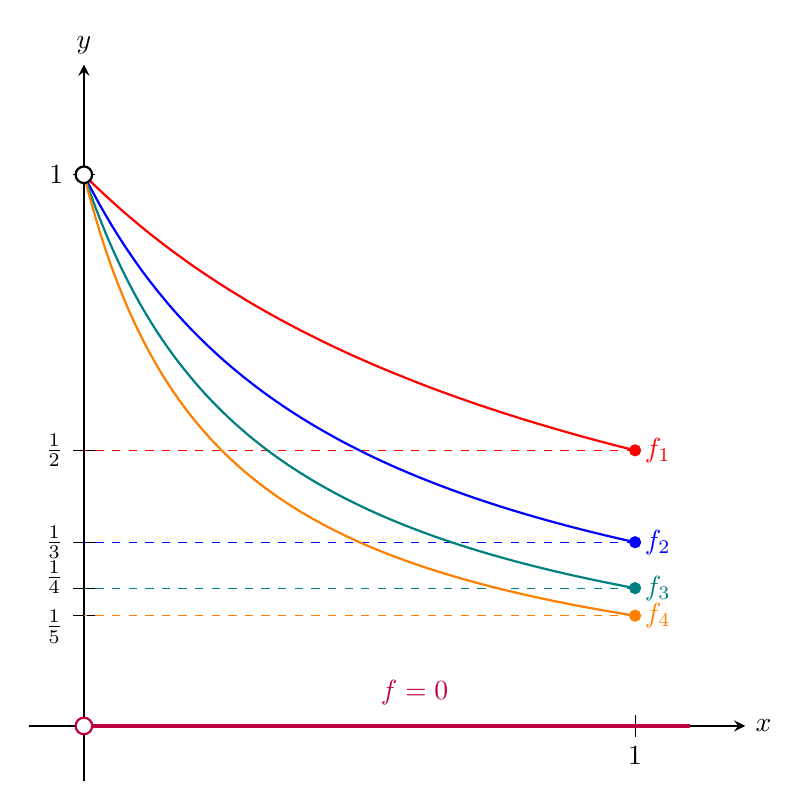
\begin{tikzpicture}[scale=7, >=stealth]
            \draw[->, thick] (-0.1, 0) -- (1.2, 0) node[right] {$x$};
            \draw[->, thick] (0, -0.1) -- (0, 1.2) node[above] {$y$};

            \draw (1, 0.02) -- (1, -0.02) node[below] {$1$};

            \draw (0.02, 1) -- (-0.02, 1) node[left] {$1$};
            \draw (0.02, 1/2) -- (-0.02, 1/2) node[left] {$\frac{1}{2}$};
            \draw (0.02, 1/3) -- (-0.02, 1/3) node[left] {$\frac{1}{3}$};
            \draw (0.02, 1/4) -- (-0.02, 1/4) node[left, yshift=4pt] {$\frac{1}{4}$};
            \draw (0.02, 1/5) -- (-0.02, 1/5) node[left, yshift=-4pt] {$\frac{1}{5}$};

            \foreach \n/\col/\yval in {
                1/red/0.5,
                2/blue/0.3333,
                3/teal/0.25,
                4/orange/0.2
            } {
                \draw[\col, thick, domain=0:1, samples=100] plot (\x, {1/(\n*\x + 1)});
                \draw[\col, dashed, thin] (1, \yval) -- (0, \yval);
                \filldraw[\col] (1, \yval) circle (0.01);
                \node[\col, right] at (1, \yval) {$f_\n$};
            }

            \draw[purple, very thick] (0.015, 0) -- (1.1, 0);
            \node[purple, above] at (0.6, 0.02) {$f=0$};

            \filldraw[fill=white, draw=purple, thick] (0,0) circle (0.015);
            \filldraw[fill=white, draw=black, thick] (0,1) circle (0.015);
        \end{tikzpicture}
    \end{center}
    Anche se prendessimo \(S = [0,1]\), cioè la chiusura per avere un compatto, non funzionerebbe comunque
    per mancanza di continuità.
}

Alternatively, we can say that the condition is
\[
    \forall \varepsilon > 0, \exists N \suchthat \forall n>N, ||f_n-f||_{\infty, E} < \varepsilon
\]
We should say that the difference
\[
    |f_n(x) - f| \leq \varepsilon
\]
but since this must hold for all \(x\), we can use the supremum.
Questo è come dire che il limite della successione
\[
    \lim_n \left(\sup_{x\in S} |f_n(x) - f(x)\right) = 0
\]

\sproposition{Criteri convrgenza uniforme}{
    Supponiamo che esista una successione \(\{g_n\}\) e \(C>0\) tale che
    \[
        \sup_{x\in S} |f_n(x) - f_m(x)| \leq C \cdot \sup_{x\in S |g_n(x) - g_m(x)}|
    \]
    Allora se \(\{g_n\}\) converge uniformemente, anche \(\{f_n\}\) converge uniformemente.
    Viceversa, se troviamo una successione di punti \(\{x_n\} \subseteq S\)
    tali che
    \begin{align*}
        \lim_n |f_n(x_n) - f(x_n)| > 0
    \end{align*}
    Allora \[
        \sup_{x\in S} |f_n(x) - f(x)| \geq |f_n(x_n) - f(x_n)|
    \]
    cioè il supremum è sicuramente maggiore dell'espressione valutata in un singolo punto.
    In questo caso \(\{f_n\}\) non converge uniformemente.
}

\sdefinition{Spazio funzioni continue limitate}{
    \[
        C_b(S) = \{
            f \colon S \fromto \realnumbers \suchthat
            f \text{ continua e limitata}    
        \}
    \]
}

Su questo spazio abbiamo la norma
\[
    ||f||_{\infty} \triangleq \sup_{x \in S} |f(x)|
\]
Notiamo che \(||f_n-f||_\infty\) non è altro che la distanza \(d_\infty\)
indotta dalla \(||\cdot||_\infty\) sullo spazio \(C_b(S)\),
dove \(d_\infty(g, f) = ||f-g||_\infty\).

Abbiamo dimostrato complessivamente che \(C_b(S)\) è uno spazio completo.

\stheorem{}{
    \(C_b(S)\) è uno spazio di Banach rispetto alla norma infinito.
}

\sproof{}{
    Consideriamo una successione \(\{f_n\}\) nello spazio \(C_b(S)\) di Cauchy, cioè
    \[
        \lim_{m,n} d_\infty(f_n, f_m) = \lim_{m,n} ||f_n - f_m||_\infty = 0
    \]
    Vogliamo verificare che esiste quindi \(f \in C_b(S)\) tale che
    \[
        \lim_n d_\infty(f_n, f) = \lim_n ||f_n - f|| = 0
    \]
    Ma questo seguente dai risultati precedente e dalle definizioni equivalenti di convergenza uniforme.
    Infatti, il criterio di Cauchy implica
    che esista \(f \colon S \fromto \realnumbers\) tale che \(f_n\) converge uniformemente a \(f\) in \(S\).
    Inoltre, per ipotesi \(f_n\) continua e limitata.
    Quindi, \(f\) è pure continua e limitata su \(S\), cioè \(f \in C_b(S)\).
}

\stheorem{Stone-Weierstrass}{
    Sia \(S=K\) compatto.
    Allora \(\forall f \in C_b(K)\), esiste \(\{P_n\}\) successione di polinomi
    \(\realnumbers[x]\) (anche complessi) tali che \(P_n \to f\) uniformemente in \(K\).
    In altre parole, se consideriamo \(P(K)\) l'insieme dei polinomi a coefficienti reali, abbiamo che
    \(P(K)\) è denso in \(C_b(K)\) rispetto alla topologia indotta
    dalla norma infinito.
}

\subsection{Teorem di Ascoli-Arzelà}

Il seguente teorema è un analogo di Bolzano-Weierstrass, ma bisogna aggiungere una condizione.
Cerchiamo delle condizioni sulla nostra successione di funzioni che garantisca che
si possa estrarre una sottosuccessione convergente.
Oltre all'equilimitatezza ci serve l'equicontinuità.

\sdefinition{Equicontinuità}{
    Diciamo che la successione \(\{f_n\}\) è \emph{equicontinua}
    su \(S\), se \(\forall \varepsilon > 0\) esiste \(\delta(\varepsilon) > 0\)
    tale che se \(|x-y| < \delta\) per \(x,y \in S\), allora
    \[
        |f_n(x) - f_n(y)| < \varepsilon
    \]
    per \(n \in \naturalnumbers\).
}

Quindi è una sorta di continuità uniforme 
L'equicontinuità implica che \(f_n\) sia uniformemente continua su \(S\), ma non il contrario,
cioè se tutti le \(f_n\) sono uniformemente continue il \(\delta\) dell'uniforme continuità delle \(f_n\)
potrebbe dipendere da \(n\).

\sproposition{}{
    Se tutte le \(f_n\) sono lipschitziane su \(S\),
    un criterio di equicontinuità è che esista \(L > 0\) indipendente da \(n\)
    che verifica la definizione di lipschitzianità per ogni \(f_n\).
}

\sproof{}{
    Abbiamo \[
        |f_n(x) - f_n(y)| \leq L|x-y|
    \]
    e prendiamo \(\delta < \varepsilon / L\).
}

In particolare se \(f_n\) è \(\mathcal C^1\),
allora è sufficiente che \(\{f_n'\}\) sia equilimitata per garantire l'equilipschizianità,
come in analisi I.

\sproposition{}{
    Sia \(S=K\) compatto e \(\{f_n\}\) successione di funzioni continue
    su \(K\) tali che \(f_n\) converge uniformemente a \(f\) in \(K\)
    con \(f \colon K \fromto \realnumbers\).
    Allora, \(\{f_n\}\) è equicontinua.
}

\sproof{}{
    Notiamo che, visto che \(K\) è compatto, questa proposizione si lega con il fatto
    che se \(f_n\) continua su un compatto, quindi limitata, allora \(\{f_n\}\)
    equilimitata poiché converge uniformemente. % link prop
    Vogliamo mostrare che \(\forall \varepsilon > 0\)
    esiste \(\delta(\varepsilon) > 0\) tale che
    per ogni \(x,y \in K\) quando \(|x-y|<\delta\) vale
    \[
        |f_n(x) - f_n(y)| < \epsilon 
    \]
    Per la definizione di convergenza uniforme esiste
    \(N\left(\frac{\varepsilon}{3}\right)\)
    naturale tale che
    per ogni \(n \geq N\) e \(x \in K\)
    vale \[
        |f_n(x) - f(y)| < \varepsilon
    \]
    inoltre, \(f\) è limite unifome di funzioni continue,
    quindi è continua.
    Siccome è continua su un compatto, è uniformemente continua.
    Di conseguenza esiste \(\delta_0\left(\frac{\varepsilon}{3}\right)\) tale che
    \[
        |f(x) - f(y)| < \frac{\varepsilon}{3}
    \]
    per tutte le \(x,y \in K\) ove \(|x-y| < \delta_0\).
    Combinando tutto otteniamo che \(\forall n > N\)
    \begin{align*}
        |f_n(x) - f_m(y)| &\leq |f_n(x) - f(x)| + |f(x) - f(y)| + |f_n(y) - f(y)| \\
        &\leq \frac{\varepsilon}{3} + \frac{\varepsilon}{3} + \frac{\varepsilon}{3}
        = \varepsilon
    \end{align*}
    Però per dimostrare l'equicontinuità
    dobbiamo trovare un \(\delta\) che vada bene anche per \(f_1, \cdots, f_{N}\).
    Anche loro sono continue su un compatto quindi uniformemente continue.
    Di conseguenza,
    esistono \(\delta_i(\varepsilon) > 0\) tale che
    \[
        |f_i(x) - f_i(y)| < \varepsilon
    \]
    per ogni \(x,y \in K\)
    dove \(|x-y| < \delta_i\).
    Possiamo quindi prendere \(\min\{\delta_0, \delta_1, \cdots, \delta_N\}\).
}

\slemma{Lemma di Ascoli-Arzelà}{
    Sia \(S=K\) compatto e \(\{f_n\}\) una successione di funzioni equicontinua
    su \(K\) che converge puntualmente ad \(f \colon S \fromto \realnumbers\) in \(K\).
    Allora, \(\{f_n\}\) converge uniformemente a \(f\).
}

Quindi \(f\) è pure continua.

\sproof{}{
    Per il criterio di Cauchy,
    ci basta dimostrare che per ogni \(\varepsilon > 0\) esiste \(N(\varepsilon)\) naturale tale che
    \[
        \forall m,n > N,
        |f_n(x) - f_m(x)| < \varepsilon, \forall x \in K
    \]
    Dall'equicontinuità, \(\exists \delta\left(\frac{\varepsilon}{3}\right) > 0\)
    tale che \(\forall x,y \in K\) e \(i \in \naturalnumbers\)
    \[
        |x-y| < \delta \implies
        |f_i(x) - f_i(y)| < \varepsilon
    \]
    Visto che \(K\) è compatto, esistono \(x_1, \cdots, x_N \in K\)
    tale che
    \[
        K \subseteq \bigcup_{j=1}^N B_\delta(x_j)
    \]
    Visto che \(\{f_n\}\) converge puntualmente, in \(K\)
    per il criterio di Cauchy per successioni numeriche,
    \(\forall J \in \{1, \cdots, N\}\) esiste \(N_J\left(\frac{\varepsilon}{3}, x_j\right)\)
    naturale tale che
    \[
        |f_n(x_j) - f_m(x_j)| < \frac{\varepsilon}{3}
    \]
    per tutte le \(m,n > N_J\).
    Prendiamo \(\overline N = \max \{N_1, \cdots, N_N\}\).
    Combinando tutto
    \begin{align*}
        |f_n(x) - f_m(x)| &\leq |f_n(x) - f_n(x_i)| + |f_m(x_i) - f_m(x)|
        + |f_n(x_i) - f_m(x_i)|
    \end{align*}
    dove \(x_i \in K\) tale che \(x \in B_\delta(x_i)\), che esiste sempre.
    Quindi, \(|x-x_i| < \delta \) e di conseguenza
    \[
        |f_n(x) - f_m(x)| < \frac{\varepsilon}{3} + \frac{\varepsilon}{3} + \frac{\varepsilon}{3} = \varepsilon
    \]
}

\stheorem{Ascoli-Arzelà}{
    Prendiamo \(S=K\) compatto e consideriamo
    \(\{f_n\}\) successione di funzioni
    \begin{enumerate}
        \item equicontinua su \(K\);
        \item equilimitata su \(K\);
    \end{enumerate}
    Allora, esiste una sottosuccessione uniformemente convergente in \(K\).
}

\begin{snippetproof}{Ascoli-Arzelà}
    Per il lemma ci basta mostrare che esiste una sottosuccessione
    che converge puntualmente.
    Prendimo \(r_1 \in K \intersection \rationalnumbers\).
    Consideriamo la successione \(\{f_n(r_1)\}\).
    Grazie all'equilimitatezza essa è limitata, e quindi per
    Bolzano-Weierstrass esiste una sottosuccessione \(\{f_{n_k}(r_1)\}\)
    convergente. Denotiamo per comodità \(f^1_n \triangleq f_{n_k}\).
    Ripetiamo il ragionamento prendendo \(r_2 \in K \intersection \rationalnumbers\)
    diverso da \(r_1\) e consideriamo la successione \(\{f^1_n(r_2)\}_{n \in J}\)
    con \(J \subseteq \naturalnumbers\) infinito.
    Per lo stesso ragionamento di prima estratto una sottosuccessione convergente
    \(\{f^2_{n_k}(r_2)\}_{k\in\naturalnumbers}\) e denotiamo \(f^2_n \triangleq f^1_{n_k}\).
    Ripetiamo il processo all'infinito e quindi otteniamo una famiglia di sottosuccessioni
    \[
        \{f_n\} \supseteq \{f_n^1\} \supseteq \{f_n^3\} \cdots
    \]
    Consideriamo la diagonale del seguente diagramma:
    \begin{center}
        % https://tikzcd.yichuanshen.de/#N4Igdg9gJgpgziAXAbVABwnAlgFyxMJZABgBpiBdUkANwEMAbAVxiRADMB9ARgD1uQAX1LpMufIRTdyVWoxZsuAJn5CRIDNjwEiSmdXrNWiDpwDMq4aK0SiZ-XKOLOAFkvrN4nSjLdZhhRMuPiU1ay9JZGk-A3ljUxVQqw0xbUi9GMdA0wskj1TbFHtMgPiuNzzwtLtSJX845zczMJSbb2Q9OtinIPNeZuTPaqla+p6E-pahwpJR7uzgycGC9rIzMYWeXhcplcjpdfmyzhUd5bb00kOs44sz-Iua69LG7d3HlBcrjfiAHV+AMZQCA4BDnCJEL5dG5sf5AkFgh4Qz6kEoNExw4Gg97I5BfShHWGArGIqozMguH5EmgknHDKKkSmEjG-GkIukzPRMmEstnY8H0+zcl682kCmZfYXokD-KBi2QwKAAc3gRFA7AAThAALZIMggHAQJAAVmSmp1JuohqQAE4zVrdYgbVajYhuKaKIIgA
        \begin{tikzcd}
        f_1^1 \arrow[rd] & f_2^1            & f_3^1            & f_4^1  & \cdots \\
        f_1^2            & f_2^2 \arrow[rd] & f_3^2            & f_4^2  & \cdots \\
        f_1^3            & f_2^3            & f_3^3 \arrow[rd] & f_4^3  & \cdots \\
        f_1^4            & f_2^4            & f_3^4            & f_4^4  & \cdots \\
        \vdots           & \vdots           & \vdots           & \vdots & \ddots
        \end{tikzcd}
    \end{center}
    Impostiamo
    \(g_k = f_k^k\).
    Per costruzione \(\forall x \in K \intersection \rationalnumbers\)
    vale che \(\{g_k(x)\}_{k \in \naturalnumbers}\)
    converge per come abbiamo costruito
    le \(f_k^k\). Dobbiamo dimostrare che questa successione converga su tutto \(K\).
    Visto che \(\{g_k\}\)
    è contenuta in \(\{f_n\}\)
    allora è equicontinua, quindi esiste per ogni \(\varepsilon > 0\) un \(\delta\left(\frac{\varepsilon}{3}\right)\)
    tale che \[ |g_k(x) - g_k(y)| < \varepsilon\]
    per ogni \(k \in \naturalnumbers\) e per ogni \(x,y \in K\)
    quando \(|x-y| < \delta\).
    Ma per tutte le \(x \in K\) esiste \(x_0 \in K \intersection \rationalnumbers\)
    tale che \(|x-x_0| < \delta\).
    Inoltre per il criterio di Cauchy per successioni numeriche esiste \(N\left(\frac{\varepsilon}{3}, x_0\right)\)
    tale che \[
        |g_n(x_0)- g_m(x_0)| < \frac{\varepsilon}{3}, \quad \forall n,m \geq N
    \]
    Combinando il tutto ottengo che
    \begin{align*}
        |g_n(x) - g_m(x)| &\leq |g_n(x) - g_m(x)| + |g_m(x_0) - g_m(x)| + |g_m(x_0) - g_m(x_0)| \\
        &\leq \frac{\varepsilon}{3} + \frac{\varepsilon}{3} + \frac{\varepsilon}{3} = \varepsilon
    \end{align*}
    per tutte le \(n,m > N\), visto che \(|x-x_0| < \delta\).
    L'epsilon dipende da \(x\) ma noi vogliamo la convergenza puntuale.
\end{snippetproof}

\sexample{}{
    Questo teorema ha ipotesi molto forti,
    ma il risultato è tuttavia banale-
    Anche in casi ``buoni'' non è scontato poter estrarre una sottosuccssione convergente.
    Prendiamo \(S = K = [0,1]\) come dominio e
    \[
        f_n(x) = \frac{x^2}{x^2 + (1-nx)^2}
    \]
    È facile notare che questa converge puntualmente ad \(f=1\).
    Inoltre \(|f_n(x)| \leq 1\)
    e \(f_n(1/n) = 1\).
    Se esistesse una sottosuccessione
    \(\{f_n\}\) dovrebbe convergere ad \(f\), tuttavia
    \[
        \sup_{x \in [0,1]} |f_{n_k} - f| = \sup_{x \in [0,1]}
        |f_{n_k}(x)| > f_{n_k}(\frac{1}{n_k}) > 1
    \]
    che è assurdo perché il sup è sempre maggiore o uguale della funzione valutata in un punto.
}


\end{document}